\chapter{Distributed Computing}
\label{ch:spark}

Distributed computing plays a great role in this study, which is the platform for model training and stock prediction. Before starting illustrating those data mining algorithms, let’s talk about the distributed platform those method based on first.\\


In section~\ref{sec:dm_dc} reviews two popular cluster computing frameworks, MapReduce and Spark. This Chapter first simply introduces the details of these two frameworks, then makes a comparison between them and reaches to the reason why this study chooses Spark. After that, this chapter also introduces the core technology and machine learning library of Spark.


\section{MapReduce}
MapReduce can represent two different things: the programming model and the specific implementation of framework based one that model.\cite[p.~25]{sammer2012hadoop} This chapter focuses more on the former and uses Hadoop MapReduce to refer the later meaning.\\

The first idea of MapReduce was defined in a paper written by two Google engineers in 2004, titled “MapReduce: Simplified Data Processing on Large Clusters”\cite[p.~25]{sammer2012hadoop}. Developers are only need to write \emph{map} and \emph{reduce} functions, and can leave all the other things, like parallelization, distribution and fault-tolerance of work, to the framework.


\section{Spark}

Apache Spark is another popular open source cluster computing framework with the features of fast, easy to use and wide supported. Originated at the UC Berkeley AMPLab in 2009 and later contributed to the Apache Software Foundation in 2010, Spark are designed to support wider class of applications than MapReduce, while retaining its properties like fault tolerance, data locality and scalability \cite{meng2016mllib}.\\


Spark is a flexible operational framework, which ``powers a stack of libraries including SQL and DataFrames, MLlib for machine learning, GraphX, and Spark Streaming''\cite{apache_spark}. Developers can combine these libraries with Spark seamlessly.
\begin{figure}[h]
	\centering
	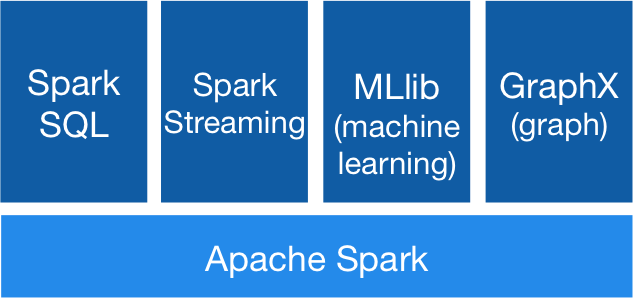
\includegraphics[width=0.8\textwidth]{spark-stack}
	\caption{Spark Stack}
\end{figure}


Spark optimizes for iterative computations, which allows users to load data to the cluster memory, and do repeated operation on these data many times, which makes it very suitable for machine learning\cite{meng2016mllib}.

\section{Comparison between MapReduce and Spark}
The simplicity of MapReduce is attractive for developers but this framework has some limitations. MapReduce is designed to batch jobs which makes it not good at iterative computations that need to run the same mapper and reducer multiple times, with output from the reducer as input to mapper of the next stage (like machine learning application)\cite{shi2015clash}. Let's use Hadoop MapReduce, a widely used implementation to describes this shortcomings. As shown in Figure~\ref{fg:hadoop}, while Hadoop MapReduce is processing computing, it need to store intermediate data into HDFS, which causes extensive data movement and duplication across the network and file system. As a result, HDFS I/O is often the bottleneck of this system.

\begin{figure}[h]
	\centering
	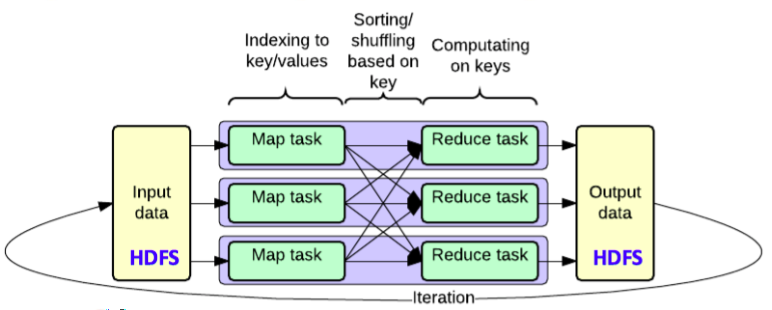
\includegraphics[width=0.9\textwidth]{hadoopcycle}
	\caption{Data cycle in Hadoop MapReduce}
	\label{fg:hadoop}
\end{figure}

From the above description, MapReduce do not have efficient data sharing method. Spark solve this problem using in-memory data processing and sharing\cite{apache_spark}. As shown in Figure~\ref{fg:spark}, Spark is based on the in-memory framework. While computing, those intermediate data is temporarily stored in memory, which greatly speed up the execution. Especially for those applications that needs iterations.

\begin{figure}[h]
	\centering
	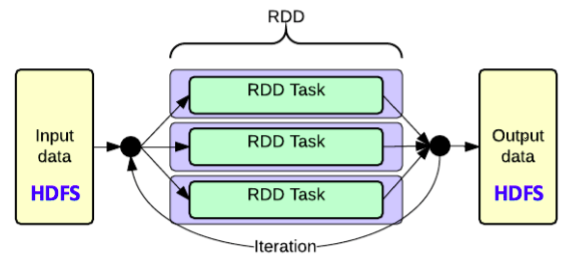
\includegraphics[width=0.8\textwidth]{sparkcycle}
	\caption{Data cycle in Apache Spark}
	\label{fg:spark}
\end{figure}

The result in contest also prove this theory. In the Daytona GraySort contest for 2014, Apache Spark wins the first price\cite{3_xin_2014}. Results can be find in table~\ref{tb:hadoop_vs_spark}. Spark sorted the same data 3X faster using 10X fewer machines.
\begin{table}[h]
	\centering
	\resizebox{\textwidth}{!}{%
		\begin{tabular}{|l|c|c|c|}
			\hline
			& \textbf{Hadoop World Record} & \textbf{Spark 100 TB} & \textbf{Spark 1 PB} \\ \hline
			\textbf{Data Size} & 102.5 TB & 100 TB & 1000 TB \\ \hline
			\textbf{Elapsed Time} & 72 mins & 23 mins & 234 mins \\ \hline
			\textbf{\# Nodes} & 2100 & 206 & 190 \\ \hline
			\textbf{\# Coes} & 50400 & 6592 & 6080 \\ \hline
			\textbf{\# Reducers} & 10,000 & 29,000 & 250,000 \\ \hline
			\textbf{Rate} & 1.42 TB/min & 4.27 TB/min & 4.27 TB/min \\ \hline
			\textbf{Rate / node} & 0.67 GB/min & 20.7 GB/min & 22.5 GB/min \\ \hline
			\textbf{Sort Benchmark Daytona Rules} & Yes & Yes & No \\ \hline
			\textbf{Environment} & dedicated data center & EC2 (i2.8xlarge) & EC2 (i2.8xlarge) \\ \hline
		\end{tabular}%
	}
	\caption{Spark TeraSort vs MapReduce\cite{3_xin_2014}}
	\label{tb:hadoop_vs_spark}
\end{table}


\section{Core Data Structure in Spark}

Resilient distributed datasets and dataframe are the basic data structure used in Spark to handle data.\\

\subsection{Resilient Distributed Datasets}

Resilient distributed datasets, or RDD, designed based on Matei\cite{zaharia2012resilient}, is one of the core technology in Spark frame. RDD can be regard as a table in database, which can hold any type of data. Spark save data to different partitions RDD.\\


Every RDD can contain many partitions, a partition is a part of dataset. RDD can rely on each other. The case that each partition of the parent RDD is used by at most one partition of the child RDD is called narrow dependency, data shuffling is unnecessary in this type of operation; while multiple child partitions may depend on one parent partition is called wide dependencies, this type of operations involves data shuffling.
\begin{figure}[h]
	\centering
	\subfigure[Narrow Dependency]{
		\centering
		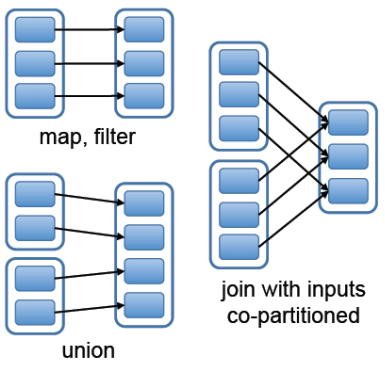
\includegraphics[width=.6\linewidth]{narrowdependencies}
	}
	\subfigure[Wide Denpendency]{
		\centering
		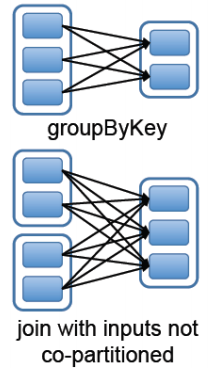
\includegraphics[width=.3\linewidth]{widedependences}
	}
	\caption{Two types of Spark Dependency\cite[p.~8]{zaharia2012resilient}}
\end{figure}

There are two reasons that why Spark make narrow dependencies out of wide one\cite[Chapter~5]{zaharia2012resilient},
\begin{enumerate}
	\item Narrow allow for pipelined execution on one cluster node, while wide dependencies must wait for all the parent partitions available.
	\item Fault recover is much easier for narrow dependencies, as it just need to re-compute the lost partitions, and this operation can be done in different nodes. On the other hand, wide dependencies involves many parent partitions.
\end{enumerate}

RDDs are immutable, the returns of every operation on RDD is a new RDD. RDD support two types of operations,

\begin{enumerate}
	\item Transformation\cite[Section~2.2]{zaharia2012resilient}: each transformation takes (one or more) RDDs, and outputs the transformed RDD (another RDD) by applying some function to the contents (e.g., map, filter, groupBy). All transformations in Spark are lazy, only computed when an action requires a result to be returned to the driver program.
	\item Action\cite[Section~2.3]{zaharia2012resilient}: Return a value to the driver program after running a computation on the dataset (e.g., reduce, reduceByKey, etc.). An action is used to either save result to some location (HDFS) or to display it via the driver program.
\end{enumerate}

To solve the problems about fault tolerance, RDD support two type of operation

\begin{enumerate}
	\item An automatic way, the RDDs log lineage (the sequence of transformations used to produce the current RDD) information\cite[Section~2.5]{zaharia2012resilient}. And when data lost happened, spark would recursively go back to the very root, or the previous checkpoint, and then re-compute the lost data.
	\item User can manually set checkpoint, at which Spark would truncated lineages and store data in reliably location, like HDFS\cite[Section~5.3]{zaharia2012resilient}.
\end{enumerate}

\subsection{Spark SQL and DataFrame}
Spark SQL was first released in May 2014. The Goal of Spark SQL is to provide an efficient, extensive and programmer-friendly API within Spark programs (on native RDDs)\cite{armbrust2015spark}.\\ 

Spark SQL runs on top of Spark. Its structure is shown in figure~\ref{fg:spark_structure}. Spark SQL provide a data structure called DataFrame (Which was first released in Spark 1.3.0 on Mar. 13, 2015. \footnote{\url{http://spark.apache.org/releases/spark-release-1-3-0.html}}). This API is similar to the data frame concept in R\footnote{The R Project, \url{https://www.r-project.org/}} and python\footnote{Python Data Analysis Library \url{http://pandas.pydata.org/}}.\\

\begin{figure}[h]
	\centering
	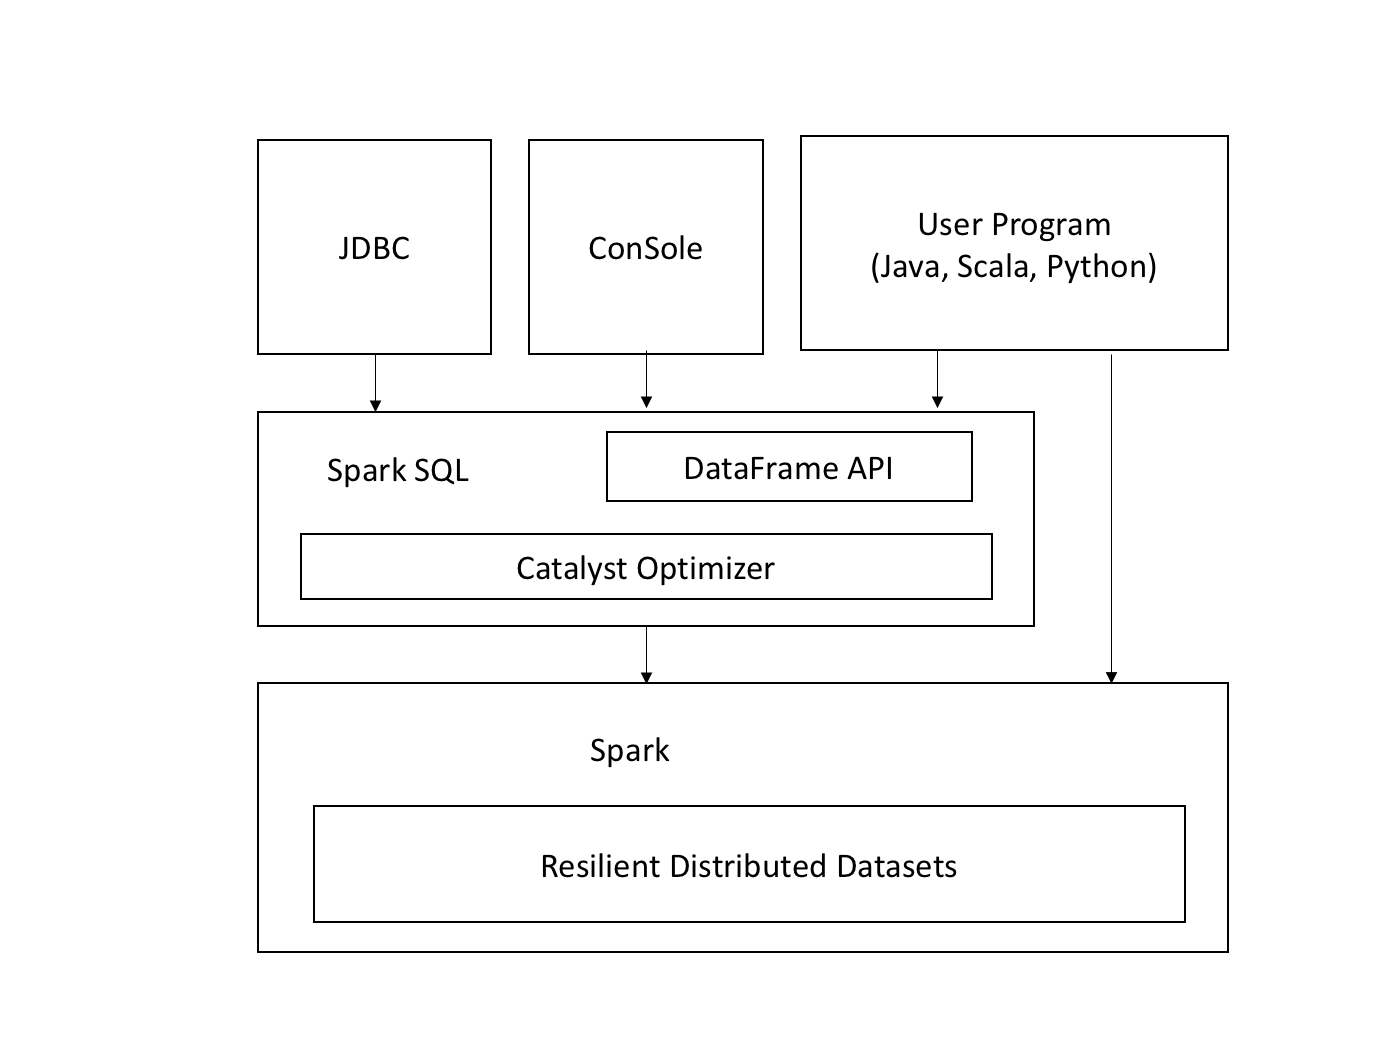
\includegraphics[width=0.8\textwidth]{DistributedSystem/Interface}
	\caption{Interfaces to Spark SQL, and interaction with Spark\cite{armbrust2015spark}.}
	\label{fg:spark_structure}
\end{figure}


Similar to RDDs, Spark DataFrames are also lazy, ``in that each DataFrame object represents a \textit{logical plan} to compute a dataset, but no execution occurs until the user calls a special '\textit{output operation}' such as \textit{save}.''\cite{armbrust2015spark}


\section{Spark Machine Learning Library (MLlib \& ML)}
Apart from the above benefits, MLlib is another reason that why we choose spark. MLlib is the extensible machine learning  library of Spark, which composes of general learning algorithm and utilities, includes classification, regression, clustering, collaborative filtering, dimension reduction and tuning section\cite{meng2016mllib}.\\


As native supported by Apache Spark, MLlib has the following benefits\cite{meng2016mllib}: First, since Apache Spark is designed for iterative applications, MLlib directly gains benefits through the improvements of Spark's low-level components. Second, the widely accepted by open-source community of Spark has also led to rapid growth and adoption of MLlib. Third, MLlib has great performances advantages over Mahout, another popular distributed machine learning library. Experiments in \cite{1_li_jiang_zhang_boesch_xiao_2015} shows that MLlib is about 7--9 times faster than Mahout in FP-growth mining problem.\\


From version 1.2, Spark MLlib was divided into two libraries, MlLib and ML\footnote{Spark Release Note 1.2.0 \url{http://spark.apache.org/releases/spark-release-1-2-0.html}}. MlLib contains the original API built on top of RDDs, while ML provides higher-level API built on top of Spark DataFrames for constructing ML pipelines.\\


Ml is more recommended by the official document, but MlLib is still being supported. This dissertation was based on both MlLib, and ML.


\section{Summary}
Apache Spark is an open source framework optimized for iterative programs, like machine learning. That is why this study chooses Spark instead of MapReduce.\\


The core technology of Spark is RDD, an immutable distributed data structure, which support two types of operation, transformation and action. RDD can be saved any type of storage, but usually is cached in memory.\\


Spark SQL offers DataFrame API, which is also lazy but more similar to data frame concept in R and Python. Compares to RDD, Spark DataFrame offers much more programmer-friendly API.\\


This study chooses MLlib because of its ease of use and tight integration with Spark.


